\chapter{Integration of Discontinuous Functions}
\label{chpt:integration}

As discussed in Section \ref{sec:ver-background}, the principal difficulty inherent in implementing the method of manufactured solutions for integral equations lies in the evaluation of the flux and volume integrals required in order to compute the manufactured source terms. Multidimensional integration is itself a difficult problem, and is made more so by the presence of discontinuities in the integrand. As the intended use of these integrals is to verify the numerical accuracy of other codes, it is important that they be evaluated as accurately as possible, which is also made more difficult by the presence of discontinuities. 

To resolve these difficulties and enable the use of integrative manufactured solutions, an n-dimensional integration routine was developed for general types of functions, and methods were devised for the tracking of discontinuities through iterated applications of one-dimensional integration. The resulting algorithm effectively removes discontinuities from the integrand, allowing the evaluation of the integrals to proceed with the level of accuracy that would be expected for a continuously differentiable integrand function.

\section{Background}
\label{sec:int-background}

Multidimensional integration routines generally belong to one of two classifications. Monte Carlo methods rely on the fact that, over many random function samples taken with the integration region, the average value of the samples will converge to the value of the integral of the function over that region. Monte Carlo methods are especially useful because the computational cost of this procedure does not increase with the dimensionality of the integral to be evaluated. There is also no additional difficulty introduced when integrating over complex integration domains, nor when integrating ill-behaved (singular, discontinuous) integrand functions. Unfortunately, convergence to the exact value of the integral is quite slow.

In contrast, quadrature methods are more complex, and generally make more assumptions about both the integration domain and the integrand function. Quadrature methods work by sampling the function at some pre-defined number of points, using the samples to fit a polynomial to the integrand, and then evaluating the integral of the polynomial. Most quadrature methods are one-dimensional in nature, but some multidimensional methods do exist.\cite{Cuba/Cubature}. Because quadrature methods use polynomials to approximate the integrand function, difficulties arise when attempting to evaluate functions that cannot easily be represented as polynomials, such as discontinuous functions. For smooth functions, quadrature typically provides excellent accuracy when compared to Monte Carlo methods.

Smoothing of integrand functions can be achieved through subdivision of the integration domain along discontinuous surfaces, resulting in a set of integrals over irregular domains where the integrand is smooth. In multiple dimensions, this process is analogous to the problem of shock-fitting, and very difficult...

Although multidimensional subdivision of integrals is difficult, the same process is straightforward in one dimension. By using one-dimensional integration routines iteratively, the problem is greatly simplified. Some tools are ... 

No available tools were able to do n-dimensional integrals, with the level of control necessary ...

Given the initial locations of any discontinuities, it is only necessary to propagate these through each level of integration in order to subdivide the integral appropriately at every level such that the resulting function is smooth.

\section{Nquad Development}
\label{sec:int-nquad}

As discussed in Section \ref{sec:int-background}, a tool needed to be developed for general n-dimensional integration using iterative application of one-dimensional quadrature. The SciPy library\cite{Oliphant2007} provided the closest such tool. The flexible nature of {\tt scipy.integrate.quad}, together with its support for multivariate functions, provided the basic functionality required for extension to n-dimensional problems, and it was selected as the baseline for development of {\tt nquad}, a general-purpose, flexible routine for the evaluation of multidimensional integrals, with access to the entire suite of {\tt Quadpack} integration tools.

Making this tool publicly available was a major focus, and a concerted effort was made to make it useful in a wide range of applications. {\tt nquad} was incorporated into the SciPy library in version 0.13, and further performance optimizations are accepted and scheduled for inclusion in version 0.15. 

\subsection{{\tt Nquad} interface and algorithm}

{\tt Nquad} was developed as a Python wrapper to {\tt scipy.integrate.quad}, following the model of the already extant {\tt scipy.integrate.dblquad} function. The internal structure is illustrated in Fig.~\ref{fig:nquad-flow-chart}. 

\begin{figure}
\centering
\label{fig:nquad-flow-chart}
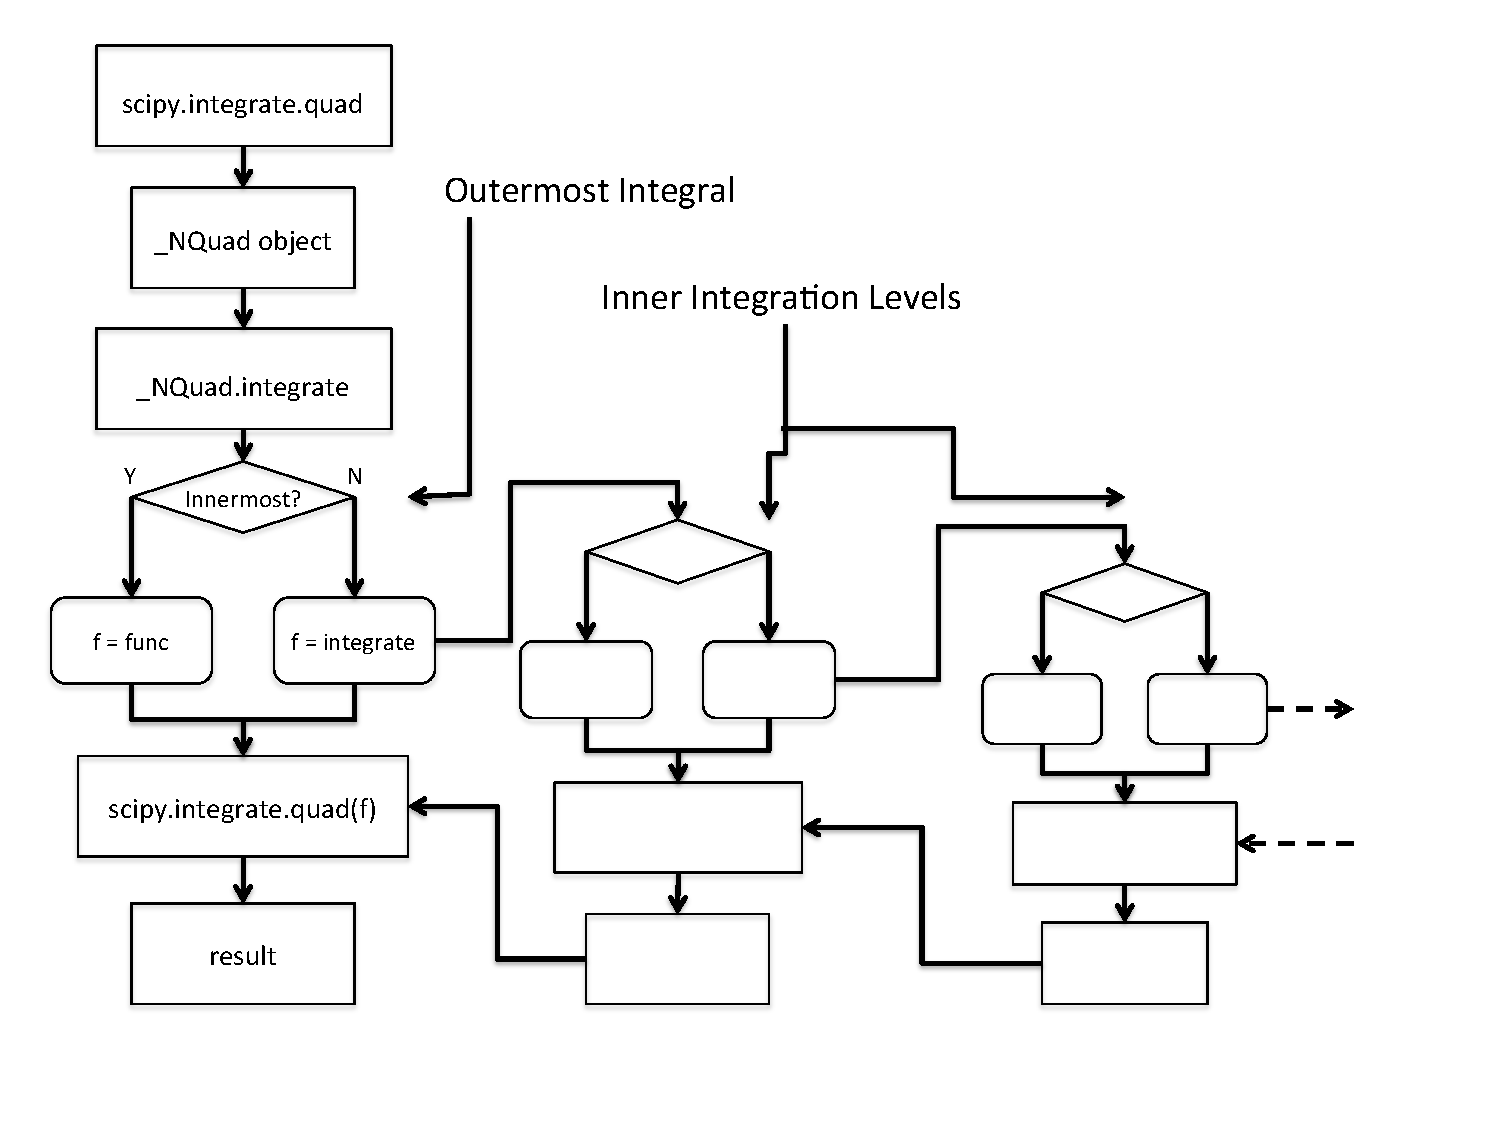
\includegraphics[width=\textwidth]{nquad_flow_chart.pdf}
\caption{The {\tt nquad} algorithm, diagrammed for 3+ dimensional integrals.}
\end{figure}

{\tt nquad} has a simple user interface that nonetheless allows for fine control of the integration processes if desired. It is called as a function of the form:

{\tt nquad(f,ranges,args,opts)}

where {\tt f} is the function to be integrated, {\tt ranges} is a list of the ranges of integration, {\tt args} is any additional arguments required by {\tt f} beyond the integration variables, and {\tt opts} contains the integration options corresponding to the underlying levels of integration. 

This interface is a simple wrapper to the underlying machinery. It processes the arguments it receives into the appropriate form, and initializes an {\tt \_NQuad} object. This object provides the {\tt integrate} method, which is called recursively to evaluate the multidimensional integral. 

Using the information contained in the {\tt \_NQuad} state, the {\tt integrate} method determines whether or not it is a call corresponding to the innermost level of integration. If it is not, then it defines a temporary integrand function, which is itself a call to the {\tt integrate} method. If it does correspond to the innermost integration level, then the temporary integrand function becomes an alias for the integrand function provided by the initial {\tt nquad} call and {\tt \_NQuad} initialization. 

Once the integrand function has been defined, it is passed on to the one-dimensional integration routine, along with the appropriate integration range and options. If the integrand is a call to {\tt \_NQuad.integrate}, then an evaluation of the integrand will result in another call to {\tt quad}, and so on until the innermost level of integration is reached. 

{\tt scipy.integrate.quad} is used as the one-dimensional integration routine. It is a flexible interface to the {\tt Quadpack} library and contains many different algorithms, the choice among which is determined by the options it receives. The two most important algorithms for the purposes of the present discussion are the default adaptive Gauss-Kronrod quadrature method, and the variant that allows for externally supplied information on internal discontinuities, singularities, and other difficulties of the integrand function\cite{netlib}. When such information is provided through the {\tt points} argument to {\tt scipy.integrate.quad}, the integration domain is subdivided at those critical points, thus controlling the difficulties associated with singularities and removing the effects of discontinuities. 

It is important to note that both integration ranges and options are defined as functions. At inner levels of integration, the function is being evaluated at specific values of the outer integration variables. These values can be used to compute values for the {\tt range} and {\tt opt} arguments corresponding to that level. This is a critical feature, as it allows integration of domains that are not hyper-cubic, and it also allows {\tt points} to be specified such that they lie on some curved hypersurface. 

\subsection{Optimizing the innermost integration level}

The nature of {\tt nquad} is such that the integrand function must be evaluated many times by the underlying Fortran library. In their simplest form, {\tt nquad} and {\tt quad} provide these integrands as Python functions with the signature {\tt f(x0,...,xn,t0,...,tm)}, where {\tt x0,...,xn} are the integration variables, and {\tt t0,...,tm} are any additional arguments which the function requires. This form is preferred in most circumstances, as it interfaces very well with the overall Python environment. However, defining the integrand as a Python function entails performance sacrifices, both due to the relatively slow evaluation of complex Python functions and the repeated callbacks to Python that must be made from within the {\tt Quadpack} integration library. Since these performance sacrifices can be severe for some problems, it is beneficial to provide the user with options for performance optimization.

The most straight-forward way to improve performance of the overall {\tt nquad} integration is by using a compiled C function for the integrand. Such a function can be optimized for performance at compile-time, and also accessed natively by the {\tt Quadpack} library, thus avoiding callbacks. This would affect function calls at the innermost level of integration, where the bulk of the function evaluations are made. 

The principal difficulty with this approach is the structure of the {\tt Quadpack} library, which is written for univariate functions only. The SciPy library worked around this limitation for Python functions, but provided no interface for doing the same with C functions. Brian Newsom, a student funded through the Discovery Learning Apprenticeship program at CU-Boulder, rewrote the interface code connecting {\tt scipy.integrate.quad} with {\tt Quadpack} during the 2013-2014 school year, to support this functionality. As a result of his work, it is now possible to improve computational performance by defining {\tt f} as a C function with the signature {\tt f(n+m,[x0,...,xn,t0,...,tm])}. This function is then compiled, loaded into Python using the {\tt ctypes} module from the Python standard library, and the resulting object can be passed to {\tt quad} or any of the functions that wrap it, including {\tt nquad}. The performance improvements from this optimization are dependent on the complexity of the integrand function. For simple integrands, 2x speedups are common. For complex integrands that benefit from aggressive compile-time optimization, 10x speedups are more typical.

\section{Discontinuity tracking}
\label{sec:int-disc-tracking}

As discussed in Section \ref{sec:int-background}, the principal requirement of any multidimensional integration routine for use in code verification through the integrative method of manufactured solutions is highly accurate evaluation of integrals of discontinuous functions. Monte Carlo methods are insufficiently accurate for this purpose, and quadrature methods do not accurately capture discontinuous behavior. Subdividing the integration domain avoids this issue, but is difficult to achieve in multiple dimensions. Subdivision is much simpler if the multidimensional integrals are expressed as iterated one-dimensional integrals using Fubini's theorem. 

The key to understanding domain subdivision for iterated integrals is to recognize that each one-dimensional integration yields a new function. For example, one may consider the integration of a paraboloidal step function in three-dimensional space, given by:
\begin{equation}
% MathType!MTEF!2!1!+-
% faaagCart1ev2aaaKnaaaaWenf2ys9wBH5garuavP1wzZbqedmvETj
% 2BSbqefm0B1jxALjharqqtubsr4rNCHbGeaGqiVu0Je9sqqrpepC0x
% bbL8FesqqrFfpeea0xe9Lq-Jc9vqaqpepm0xbba9pwe9Q8fs0-yqaq
% pepae9pg0FirpepeKkFr0xfr-xfr-xb9Gqpi0dc9adbaqaaeGaciGa
% aiaabeqaamaabaabaaGcbaGaamOramaaBaaaleaacaaIWaaabeaakm
% aabmaabaGaamiEaiaacYcacaWG5bGaaiilaiaadQhaaiaawIcacaGL
% PaaacqGHHjIUdaGabaqaauaadeqacmaaaeaacaaIXaaabaGaai4oaa
% qaaiaadIhadaahaaWcbeqaaiaaikdaaaGccqGHRaWkcaWG5bWaaWba
% aSqabeaacaaIYaaaaOGaeyOeI0IaamOEaiabgYda8iaaicdaaeaaca
% aIWaaabaGaai4oaaqaaiaadwgacaWGSbGaam4CaiaadwgaaaaacaGL
% 7baaaaa!47CC!
{F_0}\left( {x,y,z} \right) \equiv \left\{ {\begin{array}{*{20}{c}}
1&;&{{x^2} + {y^2} - z < 0}\\
0&;&{else}
\end{array}} \right.
\label{eq:int-paraboloidal-step}
\end{equation}
Assuming that this function is integrated, with an integration order and volume given by:
% MathType!MTEF!2!1!+-
% faaagCart1ev2aaaKnaaaaWenf2ys9wBH5garuavP1wzZbqedmvETj
% 2BSbqefm0B1jxALjharqqtubsr4rNCHbGeaGqiVu0Je9sqqrpepC0x
% bbL8FesqqrFfpeea0xe9Lq-Jc9vqaqpepm0xbba9pwe9Q8fs0-yqaq
% pepae9pg0FirpepeKkFr0xfr-xfr-xb9Gqpi0dc9adbaqaaeGaciGa
% aiaabeqaamaabaabaaGcbaWaa8qeaeaacaWGgbWaaSbaaSqaaiaaic
% daaeqaaOWaaeWaaeaacaWG4bGaaiilaiaadMhacaGGSaGaamOEaaGa
% ayjkaiaawMcaaaWcbaGaamOvaaqab0Gaey4kIipakiabg2da9maape
% dabaWaa8qmaeaadaWdXaqaaiaadAeadaWgaaWcbaGaaGimaaqabaGc
% daqadaqaaiaadIhacaGGSaGaamyEaiaacYcacaWG6baacaGLOaGaay
% zkaaGaamizaiaadIhaaSqaaiabgkHiTiaaigdaaeaacaaIXaaaniab
% gUIiYdGccaWGKbGaamyEaaWcbaGaeyOeI0IaaGymaaqaaiaaigdaa0
% Gaey4kIipakiaadsgacaWG6baaleaacaaIWaaabaGaaGOmaaqdcqGH
% RiI8aaaa!53CA!
\[\int_V {{F_0}\left( {x,y,z} \right)}  = \int_0^2 {\int_{ - 1}^1 {\int_{ - 1}^1 {{F_0}\left( {x,y,z} \right)dx} dy} dz} \]

It is then possible to define new functions based on the results of this integration:
% MathType!MTEF!2!1!+-
% faaagCart1ev2aqaKnaaaaWenf2ys9wBH5garuavP1wzZbqedmvETj
% 2BSbqefm0B1jxALjharqqtubsr4rNCHbGeaGqiVu0Je9sqqrpepC0x
% bbL8FesqqrFfpeea0xe9Lq-Jc9vqaqpepm0xbba9pwe9Q8fs0-yqaq
% pepae9pg0FirpepeKkFr0xfr-xfr-xb9Gqpi0dc9adbaqaaeGaciGa
% aiaabeqaamaabaabaaGcbaGaamOramaaBaaaleaacaaIXaaabeaakm
% aabmaabaGaamyEaiaacYcacaWG6baacaGLOaGaayzkaaGaeyyyIO7a
% a8qmaeaacaWGgbWaaSbaaSqaaiaaicdaaeqaaOWaaeWaaeaacaWG4b
% GaaiilaiaadMhacaGGSaGaamOEaaGaayjkaiaawMcaaiaadsgacaWG
% 4baaleaacqGHsislcaaIXaaabaGaaGymaaqdcqGHRiI8aaaa!43E5!
${F_1}\left( {y,z} \right) \equiv \int_{ - 1}^1 {{F_0}\left( {x,y,z} \right)dx} $
and 
% MathType!MTEF!2!1!+-
% faaagCart1ev2aqaKnaaaaWenf2ys9wBH5garuavP1wzZbqedmvETj
% 2BSbqefm0B1jxALjharqqtubsr4rNCHbGeaGqiVu0Je9sqqrpepC0x
% bbL8FesqqrFfpeea0xe9Lq-Jc9vqaqpepm0xbba9pwe9Q8fs0-yqaq
% pepae9pg0FirpepeKkFr0xfr-xfr-xb9Gqpi0dc9adbaqaaeGaciGa
% aiaabeqaamaabaabaaGcbaGaamOramaaBaaaleaacaaIYaaabeaakm
% aabmaabaGaamOEaaGaayjkaiaawMcaaiabggMi6oaapedabaGaamOr
% amaaBaaaleaacaaIXaaabeaakmaabmaabaGaamiEaiaacYcacaWG5b
% GaaiilaiaadQhaaiaawIcacaGLPaaacaWGKbGaamyEaaWcbaGaeyOe
% I0IaaGymaaqaaiaaigdaa0Gaey4kIipaaaa!423A!
${F_2}\left( z \right) \equiv \int_{ - 1}^1 {{F_1}\left( {x,y,z} \right)dy} $
One could also choose a different ordering, which might lead to the function:
% MathType!MTEF!2!1!+-
% faaagCart1ev2aaaKnaaaaWenf2ys9wBH5garuavP1wzZbqedmvETj
% 2BSbqefm0B1jxALjharqqtubsr4rNCHbGeaGqiVu0Je9sqqrpepC0x
% bbL8FesqqrFfpeea0xe9Lq-Jc9vqaqpepm0xbba9pwe9Q8fs0-yqaq
% pepae9pg0FirpepeKkFr0xfr-xfr-xb9Gqpi0dc9adbaqaaeGaciGa
% aiaabeqaamaabaabaaGcbaGaamOraiaaxcW7daWgaaWcbaGaaGymai
% aaikdaaeqaaOWaaeWaaeaacaWG4bGaaiilaiaadMhaaiaawIcacaGL
% PaaacqGHHjIUdaWdXbqaaiaadAeacaWLa8+aaSbaaSqaaiaaicdaae
% qaaOGaamizaiaadQhaaSqaaiaaicdaaeaacaaIYaaaniabgUIiYdaa
% aa!4120!
$F_{12}\left( {x,y} \right) \equiv \int\limits_0^2 {F_0dz} $

These four functions are illustrated in Fig.~\ref{fig:paraboloidal-integration}.

\begin{figure}[p]
\label{fig:paraboloidal-integration}
\includegraphics[width=\textwidth]{Nate_Combined_Integration_pics2.pdf}
\caption{Progressive steps of integration of a paraboloidal step function, showing the propagation of discontinuities.}
\end{figure}

Each of these functions may be considered as an independent entity for the purposes of integration. That is, the behavior of $F_1\left(y,z\right)$ need not be considered when evaluating the integral $\int^1_{-1}F_0\left(x,y,z\right)dx$. This means that, for the computation of $F_1\left(y,z\right)$, discontinuities can be accounted for simply by dividing the integration domain at the critical values of $x$ that lie on the discontinuous surface for the appropriate values of $y$ and $z$. 

Subdividing the integration domain in this way essentially eliminates the effect of the discontinuous surface on the computation of $F_1\left(y,z\right)$, but this new function may also be discontinuous or otherwise-ill-behaved. It is therefore to devise a method for predicting such critical surfaces in $F_1$ based on knowledge of the behavior of $F_0$ and the integration step connecting the two functions.

If critical surfaces of some function $F_0\left(x_0,...,x_n\right)$ are denoted by the functions $f_{0k}\left(x_0,...,x_n\right)=0$, then critical values of $x_0$, denoted by $x_0^*\left(x_1,...,x_n\right)$, can be found. The function $F_1\left(x_1,...,x_n\right)$ can be derived by integration of $F_0$ with respect to $x_0$, subdividing the integration domain at the critical values $x_0^*$. 

The function 
% MathType!MTEF!2!1!+-
% faaagCart1ev2aaaKnaaaaWenf2ys9wBH5garuavP1wzZbqedmvETj
% 2BSbqefm0B1jxALjharqqtubsr4rNCHbGeaGqiVu0Je9sqqrpepC0x
% bbL8FesqqrFfpeea0xe9Lq-Jc9vqaqpepm0xbba9pwe9Q8fs0-yqaq
% pepae9pg0FirpepeKkFr0xfr-xfr-xb9Gqpi0dc9adbaqaaeGaciGa
% aiaabeqaamaabaabaaGcbaGaamOramaaBaaaleaacaaIXaaabeaakm
% aabmaabaGaamiEamaaBaaaleaacaaIXaaabeaakiaacYcacaGGUaGa
% aiOlaiaac6cacaWG4bWaaSbaaSqaaiaad6gaaeqaaaGccaGLOaGaay
% zkaaGaeyyyIO7aa8qmaeaacaWGgbWaaSbaaSqaaiaaicdaaeqaaOGa
% amizaiaadIhadaWgaaWcbaGaaGimaaqabaaabaGaamiEamaaBaaame
% aacaaIWaGaciyBaiaacMgacaGGUbaabeaaaSqaaiaadIhadaWgaaad
% baGaaGimaiGac2gacaGGHbGaaiiEaaqabaaaniabgUIiYdaaaa!4A1F!
${F_1}\left( {{x_1},...{x_n}} \right) \equiv \int_{{x_{0\min }}}^{{x_{0\max }}} {{F_0}d{x_0}} $
may itself have critical surfaces, which result from one of two mechanisms. 

The first source of critical surfaces in $F_1$ is orthogonality between the surface normal of the surfaces defined by the original functions $f_{0k}$ and the initial direction of integration. That is, one can define new critical surfaces $f_{1l}\left(x_1,...,x_n\right)=f_{0k}\left(x^{**}_0,x_1,...,x_n\right)$, where $x^{**}_0$ are the zeros of $\diff{f_{0k}}{x_0}$. 

Critical surfaces can also arise from the intersection between multiple surfaces, including those that bound the integration domain. For these, one can define new surfaces by solving the intersecting surfaces together to eliminate $x_0$

As an example, consider the paraboloidal step function $F_0$ given in Eq.~\ref{eq:int-paraboloidal-step}. One critical surface in $F_1$ can be derived as 
% MathType!MTEF!2!1!+-
% faaagCart1ev2aaaKnaaaaWenf2ys9wBH5garuavP1wzZbqedmvETj
% 2BSbqefm0B1jxALjharqqtubsr4rNCHbGeaGqiVu0Je9sqqrpepC0x
% bbL8FesqqrFfpeea0xe9Lq-Jc9vqaqpepm0xbba9pwe9Q8fs0-yqaq
% pepae9pg0FirpepeKkFr0xfr-xfr-xb9Gqpi0dc9adbaqaaeGaciGa
% aiaabeqaamaabaabaaGcbaWaaSaaaeaacqGHciITaeaacqGHciITca
% WG4baaamaabmaabaGaamiEamaaCaaaleqabaGaaGOmaaaakiabgUca
% RiaadMhadaahaaWcbeqaaiaaikdaaaGccqGHsislcaWG6baacaGLOa
% GaayzkaaGaeyypa0JaaGOmaiaadIhacqGH9aqpcaaIWaGaeyO0H4Ta
% amyEamaaCaaaleqabaGaaGOmaaaakiabgkHiTiaadQhacqGH9aqpca
% aIWaaaaa!46A3!
$\frac{\partial }{{\partial x}}\left( {{x^2} + {y^2} - z} \right) = 2x = 0 \Rightarrow {y^2} - z = 0$, while the intersection of the paraboloidal surface with the bounding surfaces $x=\pm1$ yields the new surface 
% MathType!MTEF!2!1!+-
% faaagCart1ev2aaaKnaaaaWenf2ys9wBH5garuavP1wzZbqedmvETj
% 2BSbqefm0B1jxALjharqqtubsr4rNCHbGeaGqiVu0Je9sqqrpepC0x
% bbL8FesqqrFfpeea0xe9Lq-Jc9vqaqpepm0xbba9pwe9Q8fs0-yqaq
% pepae9pg0FirpepeKkFr0xfr-xfr-xb9Gqpi0dc9adbaqaaeGaciGa
% aiaabeqaamaabaabaaGcbaGaamyEamaaCaaaleqabaGaaGOmaaaaki
% abgkHiTiaadQhacqGHRaWkcaaIXaGaeyypa0JaaGimaaaa!3553!
${y^2} - z + 1 = 0$.
Critical surfaces for $F_2$ may be similarly derived, though only one new critical value emerges, defined by $z-1=0$. 

It is important to note that, although changing the order of integration has no effect on the end result, the intermediate steps may be quite different, and these differences may affect the cost of integration. For instance, if the order of integration in the above problem is changed so that the integral in $z$ is evaluated first, then the resulting function will have no discontinuities at all, as seen in Fig.~\ref{fig:paraboloidal-integration}. Since dividing an integration domain increases the computational cost of that integration by at least a factor of 2, it clearly advantageous to choose the order of integration carefully so as to eliminate critical surfaces as quickly as possible. 

\section{Integration Verification}
\label{sec:int-verification}

\section{BACL-Manufactured}
\label{sec:int-BACL-Manufactured}

Insert text here

\section{Integrative Manufactured Solutions}
\label{sec:int-IMMS}

Insert text here

\section{Future Work}
\label{sec:int-future}

Insert text here
